\chapter{Introduction \& Literature Review}
\setlength{\epigraphwidth}{4.7in}
\epigraph{Life must be lived forwards, but it can only be understood backwards.}{S\"{o}ren Kierkegaard, \textit{``The Journals of S\"{o}ren Kierkegaard''}, 1844}

%----------------------------------------------------------------------------------------------------------------------------------------------------------------------------------------------------------
\section{Introduction}
Our ability to extract insights from large diverse data sets has rapidly improved with growing computing power and sophisticated algorithms. The field of \textit{statistical learning} has emerged as a framework that ranges from simple linear regression and complex algorithmic methods \cite{james2013introduction}. A main contribution of this field is the development of modeling techniques that allow for the semi-automatic creation of complex models, with many interacting predictor variables, which are not overfit, and predict well. These developments allow for more accurate and flexible empirical models to manage complex systems. For example, in hydrology, runoff formation processes are highly variable, non-linear, and spatially heterogeneous, which creates a challenge for predicting processes such as streamflow \cite{dooge1986looking}. The International Association of Hydrological Sciences (IAHS) dubbed the 2003-2012 years the decade on Predictions in Ungauged Basins (PUB) \cite{sivapalan2003iahs}. The PUB initiative has aimed the scientific community, in a coordinated manner, towards achieving major advances in the capacity to make predictions in ungauged basins (Figure \ref{fig:pubproblem}).

\begin{figure}
	\centering
	\begin{subfigure}{.5\textwidth}
		\centering
		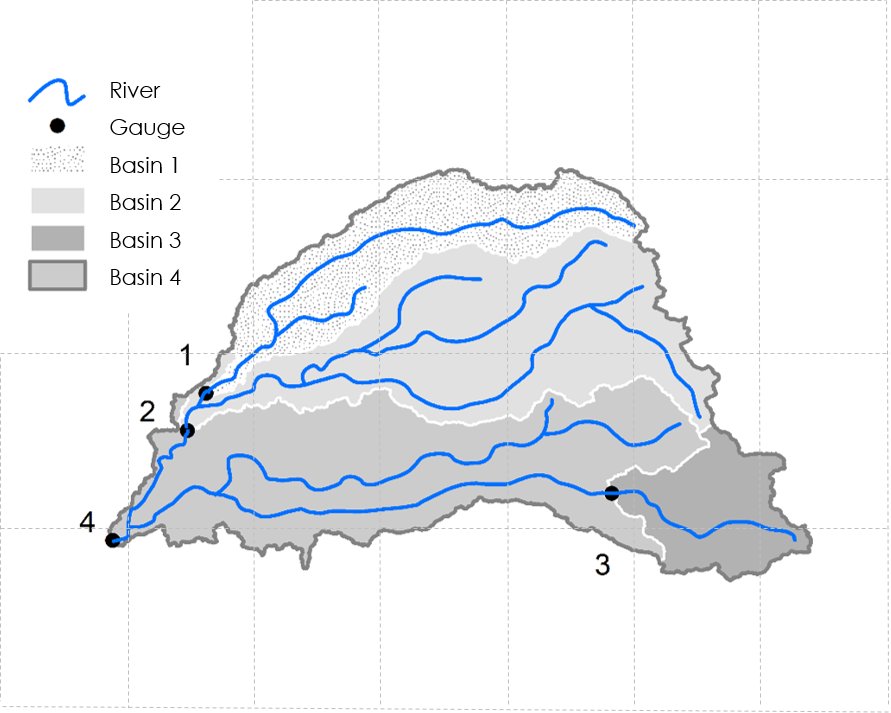
\includegraphics[width=\linewidth]{plots/ch1_pub_problem.png}
		\caption{PUB Problem}
		\label{fig:sub2}
	\end{subfigure}%
	\begin{subfigure}{.5\textwidth}
		\centering
		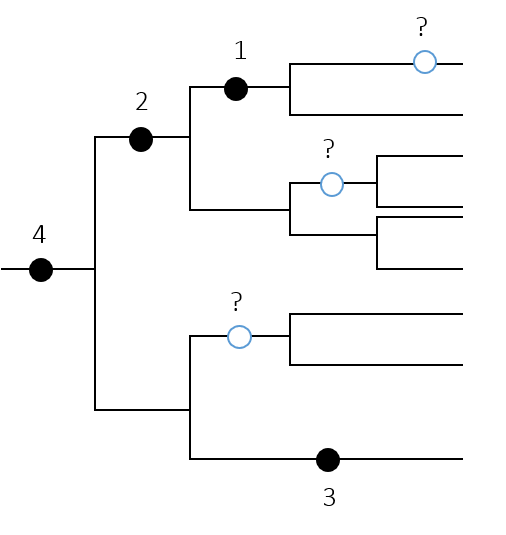
\includegraphics[width=0.74\linewidth]{plots/ch1_pub_schematic.png}
		\caption{PUB Schematic}
		\label{fig:sub1}
	\end{subfigure}
	\caption{The predicting ungauged basins (PUB) problem. This dissertation focuses on predicting unimpaired flows at ungauged locations from other gauges on the network. Predictor variables include climate and basin characteristics.}
	\label{fig:pubproblem}
\end{figure}

Predicting and forecasting hydrology at ungauged sites promotes better management of water and the environment \cite{sivapalan2003iahs}. It is
important for the sustainable management of river basins, integrating economic, social and environmental perspectives \cite{sivapalan2003prediction}, flood protection, water supply and drought management, solving water quality issues \cite{hrachowitz2013decade}, and to serve as inputs for other models. 

%----------------------------------------------------------------------------------------------------------------------------------------------------------------------------------------------------------
\section{Terms \& Definitions}
This dissertation investigates the relationships between the response variable: ``unimpaired flow'' and the predictor variables: climate and basin characteristics. Before continuing, it is useful to know how unimpaired flow is defined. Unimpaired flow is the flow that is produced by the basin in its current state, but, without dams and diversions \cite{cadwruf2016}. Unimpaired flow calculations are used mostly in places where dams have created major changes to the natural flow regime. It is often calculated by a simple accounting of water in the system (Figure \ref{fig:unimpairedflow} and Equation \ref{eq:massbalance}).
\begin{equation}
	\label{eq:massbalance}
	q_{uf} = q_{out} - q_{imp} + q_{div} + \Delta S + q_{evap}
\end{equation}

Where $q_{uf}$ is unimpaired flow, $q_{out}$ is observed gauge data, $q_{imp}$ is imported flows, $q_{div}$ is diverted flows, $\Delta S$ is the change in storage, and $q_{evap}$ is the evaporation out of the system.  

\begin{figure}
	\centering
	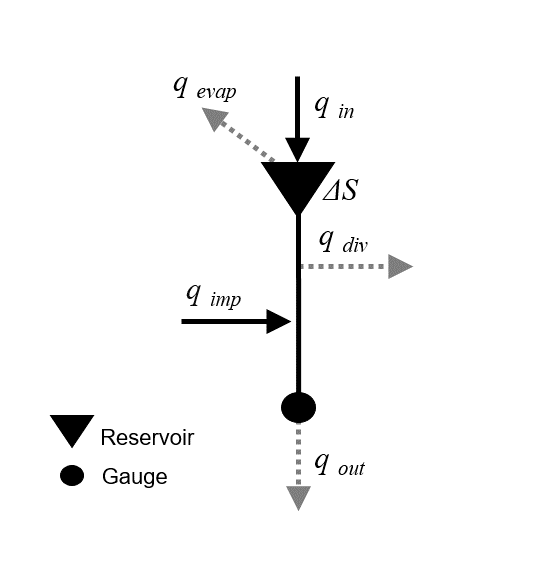
\includegraphics[width=7cm,trim={0 1cm 0 1cm},clip=true]{plots/ch1_unimpaired_flow.png}
	\caption{Calculating unimpaired flow. Unimpaired flow is calculated by adding back in diversions, subtracting imports, accounting for change in storage and evaporation caused by the reservoir.} 
	\label{fig:unimpairedflow}
\end{figure}

In contrast, ``natural flow'' is the runoff produced by a basin in its pre-development state prior to any human alterations \cite{poff1997natural}. The differences between unimpaired flow and natural flows are usually driven by effects of levees, upland land use, wetlands, and groundwater. This study, however, was only concerned with unimpaired flow; the models were built with unimpaired flow data from the California Data Exchange Center (CDEC), and the predictor variables are taken from various sources discussed in appendix \ref{a:data}. See appendix \ref{b:terms} for terms and concepts used in statistical learning. 

%----------------------------------------------------------------------------------------------------------------------------------------------------------------------------------------------------------
\section{Literature Review}

%-----------------------------------------------------------------
\subsection{Hydrologic Modeling}
Hydrologic models in PUB can be classified as \textit{mechanistic} (physical process-based, causal) or \textit{empirical} (statistical, purely stochastic) \cite{guisan2000predictive} (Figure \ref{fig:hydmodelclasses}). All modeling techniques assume that the past is a reasonable guide to the future, and that data from one basin is a useful guide to understanding hydrological responses at another basin \cite{sivapalan2003prediction}. But, each approach sacrifices some generality, realism, cost, and precision for better understanding, predicting, and managing natural resources \cite{levins1966strategy, klemes1982empirical}. 

 \begin{figure}
	\centering
	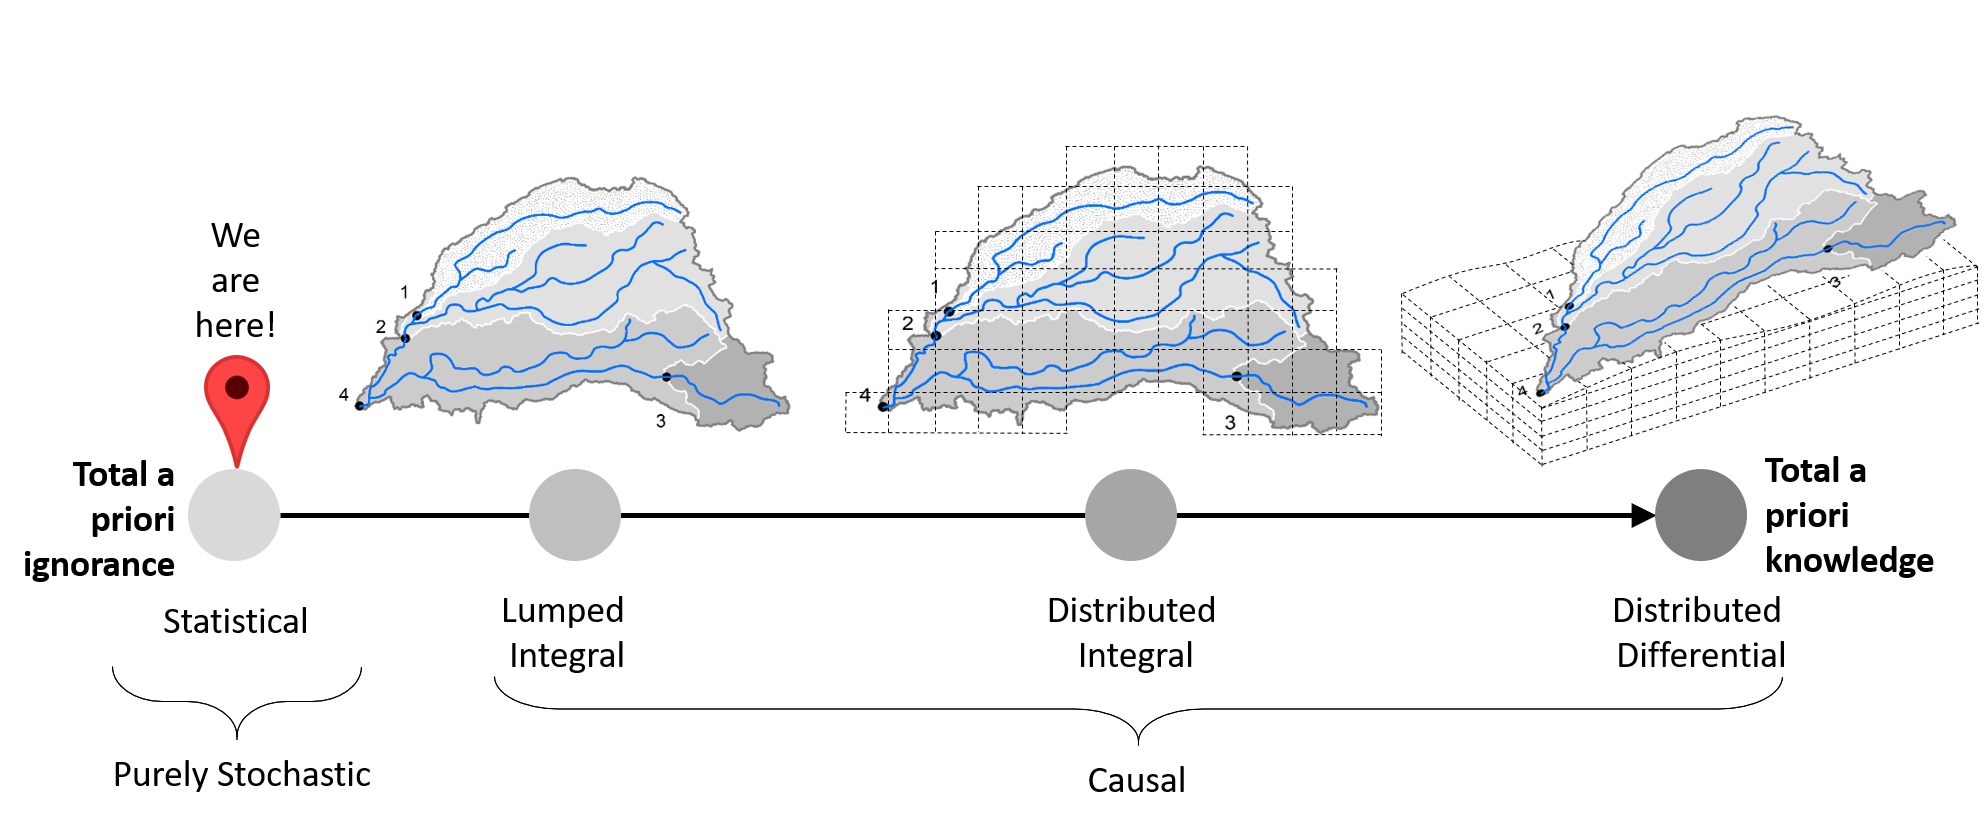
\includegraphics[width=16.51cm,trim={0 0 0 1.75cm},clip=true]{plots/ch1_hyd_model_classes.png}
	\caption{The different classes of hydrologic models. The hydrologic modeling field has been moving from total a priori ignorance to total a priori knowledge of the system. With the increase in computing power and the development of statistical learning methods, hydrologist can now re-visit predicting hydrologic conditions with purely stochastic methods.} 
	\label{fig:hydmodelclasses}
\end{figure}

Hydrologists have used both mechanistic and empirical models to capture complex runoff processes; since the mid-19\textsuperscript{th} century, with the employment of the \textit{rational method}, empirical relationships have been used in rainfall-runoff modeling \cite{beven2011rainfall}. Engineers developed the rational method in response to problems in which the design discharge was of major concern (i.e., urban sewer, land reclamation drainage systems, and reservoir spillway design) \cite{todini1988rainfall}. This method, based on the concept of concentration time, calculates runoff by simply multiplying a runoff coefficient by rainfall intensity and the basin's drainage area. It is applicable only to small or mountainous catchments where the rainfall duration normally exceeds the basin's concentration time, the time it takes for the entire basin area precipitation to reach the basin's outlet as discharge. 

To address more complexities in rainfall duration, basin size, and non-uniform characteristics, other methods emerged. In the 1930s, the \textit{unit hydrograph} method was developed \cite{sherman1932streamflow}. In the 1950s, mathematical techniques such as Z, Laplace or Fourier transforms led to the derivation of response functions from the analysis of input and output data \cite{dooge1973linear}. In the 1960s, grander approaches emerged to model the physical processes of the hydrologic cycle. Models increased in complexity over time and often lacked realistic parameter estimates, leading researchers to other ambitious mechanistic modeling efforts \cite{todini1988rainfall}. These models require considerable field input data collection and model calibration to obtain basin-specific parameters \cite{singh2005watershed}. Unfortunately, as mechanistic models increase in complexity, it is unclear if hydrologic predictions improve commensurately \cite{beven2011rainfall}. 

Our incomplete understanding of the process \cite{hrachowitz2013decade}, poor understanding of where water goes when it rains, what flow path it takes to the stream, and the age of the water that emerges in the channel \cite{sivapalan2003prediction} make PUB a difficult problem to model. Spatio-temporal heterogeneity of climate and basin characteristics create a \textit{uniqueness-of-place} issue, and there is a lack of agreement on what is a suitable regionalization technique for this problem  \cite{hrachowitz2013decade}. 

Without a unifying approach, and considering the increasing availability of environmental data, in the past two decades, more sophisticated statistical learning models have been applied to rainfall-runoff modeling. In juxtaposition with physical or semi-physical models, machine learning models learn from the data itself, with no assumptions as to the underlying process.

%-----------------------------------------------------------------
\subsection{Statistical Learning}
Artificial intelligence has gone through the ages of speculation (1940s), dawn, business, and bulldozer age \cite{winston2010class}. In the bulldozer age, with seemingly unlimited computing capacity, machines process more abundant data much like a bulldozer processes soil. Recent advances in reinforcement learning, one-hot learning (where machines learn from the first example), learning in sparse spaces, and the integration of thinking, perception, and action (rather than viewing them separately) are moving us away from the bulldozer era \cite{winston2010class}. See appendix \ref{c:history} for a brief history of statistical learning. However, the application of these newer techniques to water resources problems is slow. 
%Therefore, the literature reviewed in Section \ref{mlinciveng} is solely on computationally-intensive methods. 

% Theorists in statistical learning have made progress in developing methods, especially in supervised machine learning. However, if a statistical learning method works particularly well for one data set, it may be that the problem was defined in a space rich with solutions \cite{winston2010class}. That is, other statistical learning methods also could produce good results. Therefore, the merits of finding a solution may be due to either the statistical learning method or the problem's characteristics. Researcher can apply multiple statistical learning methods. 

We can group the statistical learning methods developed in the bulldozer age into seven main categories: \textit{supervised machine learning}, \textit{regression family}, \textit{time series analysis}, \textit{geostatistics}, \textit{multi-variate analysis}, \textit{unsupervised machine learning}, and other methods. Supervised machine learning methods are more generally used for predicting a variable in the past where no equation is needed to represent the model. In contrast, the regression family of methods are used when the purpose is more \textit{inference} than \textit{prediction}, and equations, or more specifically the coefficients of the variables in the equations, are of interest. Time series analysis is most suited to prediction problems where the time component is of interest (e.g., problem of extrapolating to the future), as opposed to geostatistics, which is mainly concerned with the spatial component of the data. Under pattern recognition problems sets, multi-variate analysis and unsupervised machine learning methods find natural groupings in the data. Other methods handle networks, text, patterns caused by latent factors, and relationships between variables, which generally don't apply to problems in water resources. Lastly, in descriptive methods, we use measures of center (e.g., mean and median), measures of spread (e.g., range, standard deviation, and quantiles), and the distribution of a variable as a way to describe the data. 

Taxonomies, like the one shown in Figure \ref{fig:modelsel}, help guide the user through a discovery process. Its goal is for the user to be able to identify an object of interest without prior knowledge of its existence. In statistical learning, method or model selection is iterative and should follow the \textit{generate-and-test} approach. So, any guide to model selection should be considered only a heuristic, meaning as a general rule it will recommend appropriate methods, but may fail sometimes. 

%\afterpage{% Insert after the current page
%	\clearpage
%	\KOMAoptions{paper=25.5in:11in,pagesize}
%	\recalctypearea
%
%	\begin{figure}
%		\centering
%   		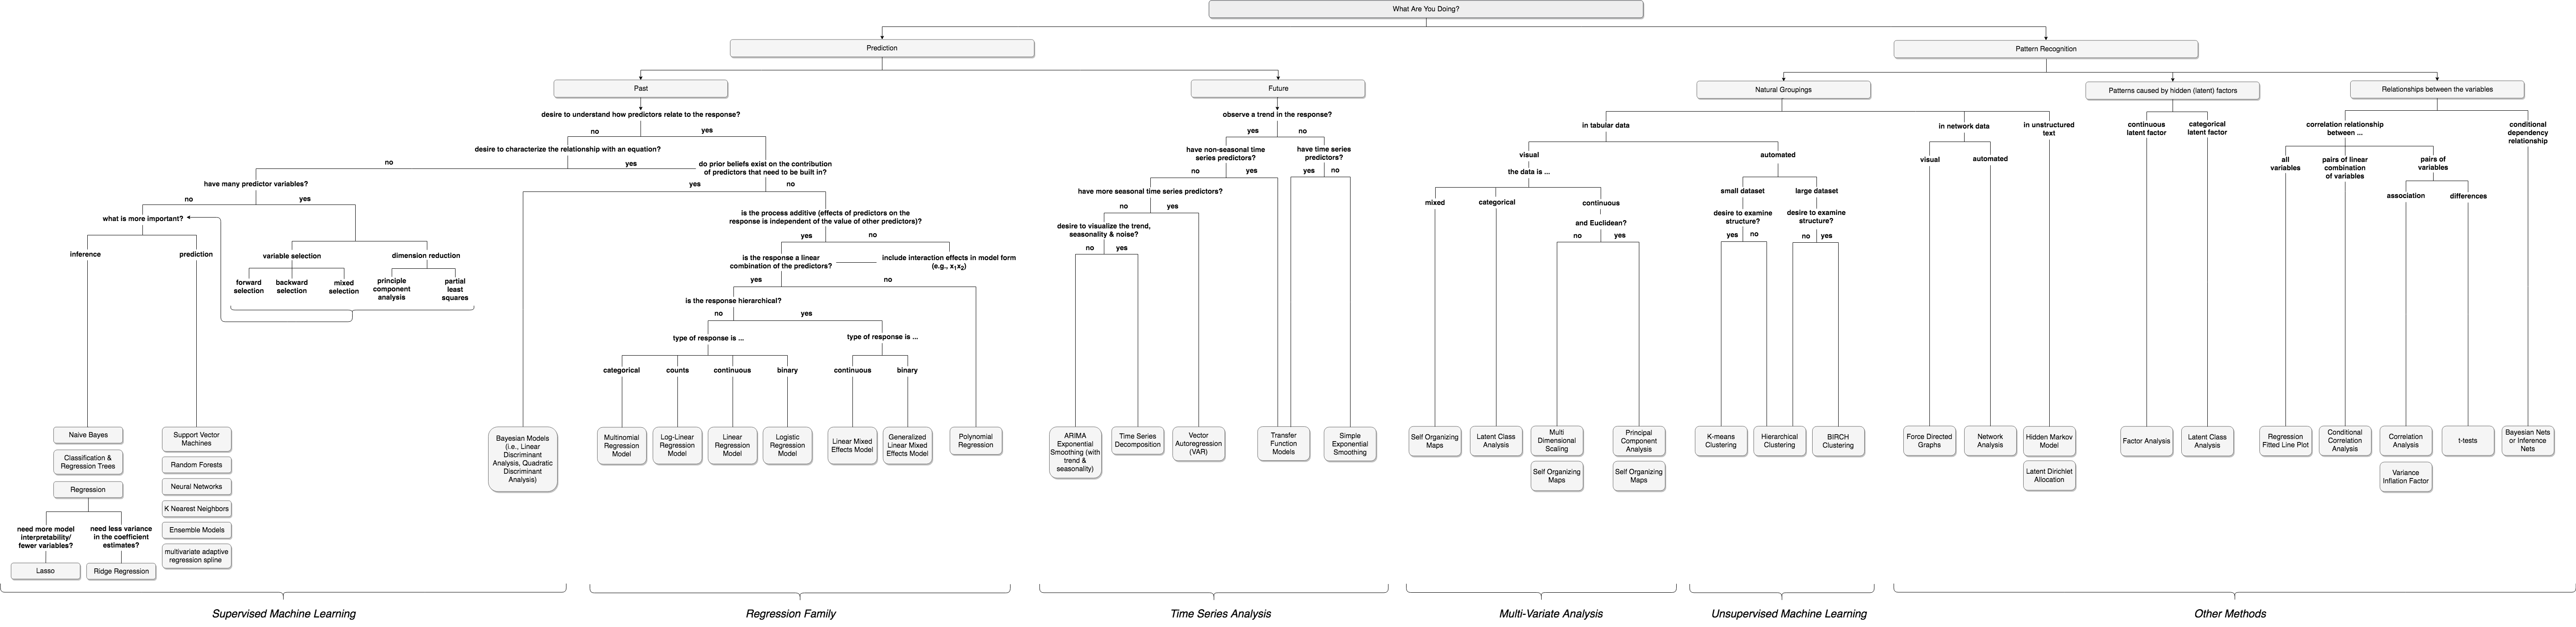
\includegraphics[width=25.5cm,trim={0 0 0 0},clip=true,keepaspectratio]{plots/model_selection.jpg}%
%   		\caption{What are you trying to do?} 
%		\label{fig:modelsel}
%	\end{figure}
%
%	\clearpage
%	\KOMAoptions{paper=A4,pagesize}
%	\recalctypearea
%}

%\begin{figure}[p]
%    \vspace*{-1in}
%    \makebox[\linewidth]{
%        \includegraphics[width=1.3\linewidth]{plots/model_selection_pages.pdf}
%    }
%    \caption{What are you trying to do? Heuristic guide for model selection.}
%\end{figure}

\begin{figure}
	\centering
	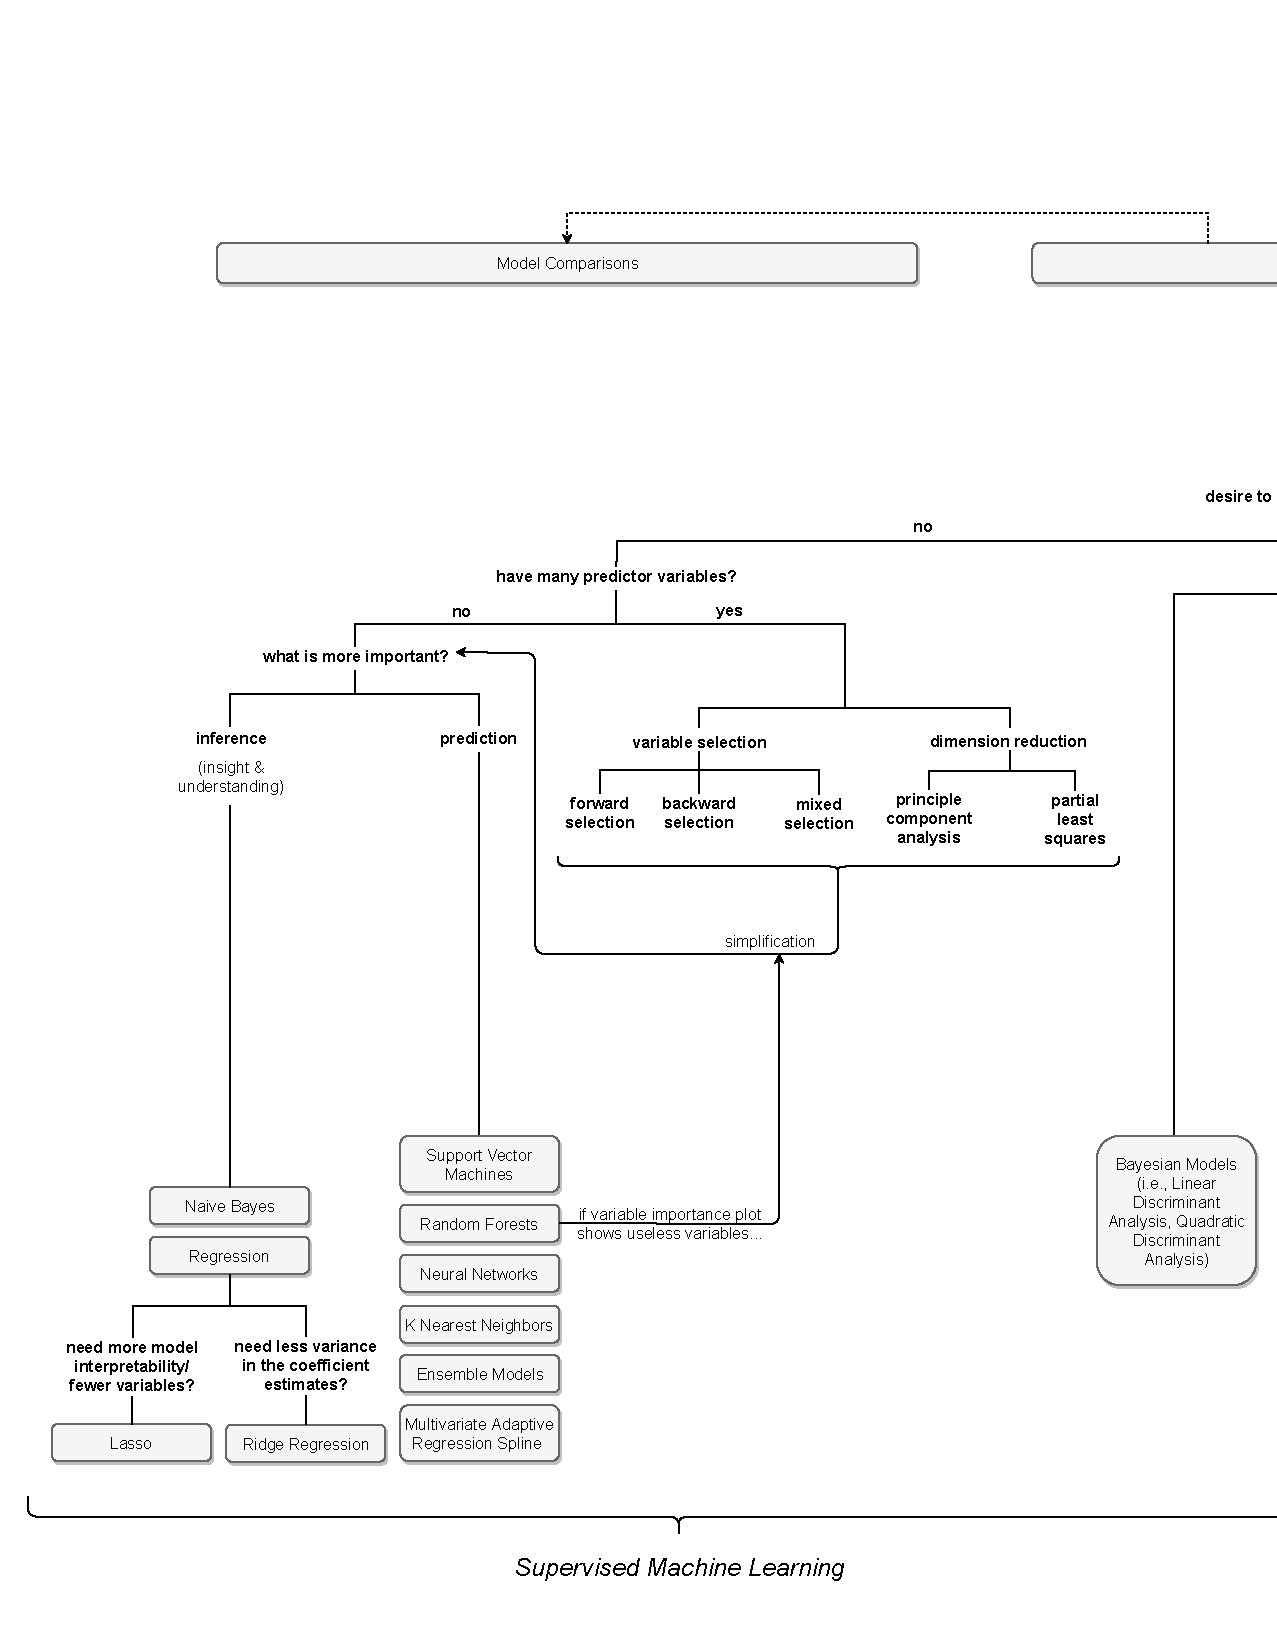
\includegraphics[width=\linewidth,trim={0 0.5in 0 0.8in},clip=true, page=1]{plots/ch1_statsflowchart.pdf}
	\caption{What are you trying to do? Heuristic guide for model selection.} 
	\label{fig:modelsel}
\end{figure}

The hydro-informatics literature shows that the techniques presented in the heuristic guide are aiding civil engineers in the fields of: (1) hydrology: e.g., rainfall-runoff modeling and model calibration; (2) hydraulics: e.g., water levels in channels and reservoirs; (3) environmental water quality: e.g., temperature and groundwater heads; (4) urban water supply: e.g., water demand and water distribution networks; and (5) general data cleaning and anomaly detection. In the following sections, we will discuss the models suitable to the PUB problem. 

%-----------------------------------------------------------------
% \subsection{Statistical Learning in Civil Engineering} \label{mlinciveng}
% CHANGE THIS WHOLE SECTION, SO IT IS ORGANIZED BY IDEAS NOT PEOPLE!!!!!!!

%Possible applications of statistical learning methods in water resources include the following: %CITATIONS COMING!!!
%
%\begin{itemize} % citations where available
%	\item Rainfall-runoff modeling: streamflow dis-aggregation or forecasting 
%	\item Building an assisting surrogate model in calibration of a rainfall-runoff model
%	\item Auto-calibration and uncertainty estimation methods
%	\item Modeling river stage-discharge relationships
%	\item Cleaning up anomalies in data: (cite Nate Chaney's work with SSURGO,  step like patterns in temperature from rounding observed data.) 
%	\item Simulating runoff, sediment and nutrient loadings from a watershed
%	\item Modeling rainfall-runoff processes intelligent controller for realtime management
%	\item Control of water levels in channels
%	\item Model-based optimal control of a reservoir
%	\item Forecasting the groundwater heads in an aquifer
%	\item River temperature prediction
%	\item Rainfall forecasting
%	\item Water demand forecasting
%	\item Flood forecasting
%	\item Predicting scour depth at culverts
%	\item Pipe deterioration models
%	\item Optimizing operations of a water distribution network 
%\end{itemize}

% rainfall-runoff modeling
% Can you break up these citations to provide a little more info about their contributions? If not, I would actually suggest reducing the list to only the most essential citations, since the others don't add much understanding. deleted: dibike1999encapsulation, abrahart2000comparing 
%As \shortciteA{solomatine2008data} explain, most machine learning techniques applied to the rainfall-runoff problem use neural networks \cite{govindaraju2013artificial}. Other studies use support vector machines \cite{lin2006using} and tree based algorithms \cite{galelli2013tree}. 
%
%% As \shortciteA{solomatine2008data} explain, most machine learning techniques applied to the rainfall-runoff problem use neural networks \cite{minns1996artificial, dawson1998artificial, tokar1999rainfall, hsu2002self, hu2007rainfall, abrahart2007timing, govindaraju2013artificial}. Other studies use support vector machines \cite{asefa2006multi, lin2006using}, and tree based algorithms \cite{iorgulescu2004nonparametric, galelli2013tree, bonniethesis}. 
%
%% flood forecasting
%\citeA{han2007flood}, \citeA{yu2004ec}, and \citeA{bray2004identification} used \textit{support vector machines} (SVMs) for flood forecasting. The applications of SVM in regression of time series is still in its infancy. Such studies show that advances are putting SVMs generally on par with neural networks in terms of model performance. 
%
%\citeA{han2007flood} shows a peculiar behavior of the SVM where lighter rainfall would generate unrealistic hydrographs that would increase to an equilibrium point rather than having the characteristic skewed bell shape. This contradicts the physical principle that limited rainfall cannot generate an unlimited flow. However, the model performs well given the data it has trained and was tested on \cite{han2007flood}. 
%
%\citeA{yu2004ec} used SVMs for real-time hydrologic forecasting. In this study, 16 years of daily data informs the learning or phase space reconstruction and the last year of record is used for a 1-lead day prediction. One problem with SVMs is their difficulty in dealing with a large training record, which is required in chaotic time series analysis. To make SVMs more suitable to such problems, a decomposition method can be applied, which is demonstrated \cite{yu2004ec}. 
%
%\citeA{bray2004identification} explored the relationships among various model structures, kernel functions (e.g., linear, polynomial, radial basis, and sigmoid), scaling factor, model parameters (i.e., cost C and epsilon) and composition of input vectors in the development of the SVM. 
%
%\citeA{gautam2001rainfall} proposes an adaptive neuro-fuzzy system with autoregressive exogenous input (ARX) structure which was capable of reasonably producing the hydrograph shape and was able to maintain a good representation of the overall water balance as well as the general flow pattern. Its excellent performance for one-step prediction shows that it will be very valuable for real-time forecasting and control of floods \cite{gautam2001rainfall}.

%% decision making
%\citeA{ames2005using} used \textit{Bayesian networks} to model water management decisions in complying with phosphorous loadings in a river. This study estimated the probability of meeting legal water quality requirements for phosphorus in a creek under several management scenarios and estimated the probability of increased recreational use of the reservoir on the creek and subsequent revenue under these scenarios. The Bayesian networks framework served as a structured means for capturing the probability that management activities will have the desired effect \cite{ames2005using}.
%
%% uncertainty estimation
%\citeA{shrestha2009assessing} used the UNcertainty Estimation based on Local Errors and Clustering (UNEEC) method for assessing total model uncertainty (i.e., model error in reproducing observed historical river flow data). The UNEEC method is a data driven technique that consists of clustering, estimation of the probability distribution of error, and building the model of the probability distribution of error \cite{shrestha2009assessing}.
%
%% time series forecasting
%\citeA{alvisi2007short} used an auto-regressive moving average (ARMA) model to forecast water demand. Since operational decisions have to be based on the
%expected future demands for water, rather than just the present known requirements, it is necessary to develop a short-term, demand-forecasting procedure. Trends, seasonality, and general periodicities are usually found in these type of time-series, which make them ideal candidates for ARMA models. 

%-----------------------------------------------------------------
\subsection{Suitable Statistical Modeling for Hydrologic Data}

Precipitation feeding into a stream needs to satisfy soil moisture deficits along its flow path before it produces runoff. In other words, the soil needs to ``fill" up to a certain threshold before it can ``spill" \cite{spence2006hydrology}. Therefore, a \textit{threshold behavior} is frequently discussed as influencing local, hillslope and catchment scale runoff generation processes \cite{zehe2008threshold}. This physical phenomenon may be why most successful machine learning techniques currently applied to the rainfall-runoff problem use artificial neural networks (e.g., \citeNP{minns1996artificial, dawson1998artificial, tokar1999rainfall, hsu2002self, hu2007rainfall, abrahart2007timing, govindaraju2013artificial}). In artificial neural networks, at each node the weighted sum of all inputs are passed through a non-linear activation function. Much like the neurons in our brains, there is a threshold that determines if the neuron will ``fire". 

The same effect can be replicated with tree based algorithms where models are built with a series of binary splits on the predictor variables (e.g., \citeNP{iorgulescu2004nonparametric, galelli2013tree, bonniethesis, worland2018improving}). Papers in which the number of basins in the study are fairly small suffer when forming the test/train or calibration/validation split. Usually, in these studies the data for one whole basin is not held out when training; in other words, the models are able to learn from a partial record from the basin of interest. Although this approach seems to be valid for rainfall-runoff modeling in the current literature, it does not comply by the test set requirements in the PUB problem where no data from the basin in the test set is available to the model. In contrast, when the datasets are large (e.g., studies done on the the GAGESII dataset, a massive USGS hydrologic data set), this problem is less pronounced. Some studies employ a random test/train split which is not appropriate when the dataset is correlated. We will discuss this concept further in chapter \ref{ch4:resampling}. These studies also employ a pre-modeling split on the dataset when classifying basins as ``impaired" vs. ``reference" basin. This imposes a subjective top split in the data and homogenizes the basins in the study; the reference basins are usually smaller headwater basins with low flows. As such, and rightly so, these models fail to make accurate predictions when extrapolating to basins lower in the network, with higher flows, since the model was denied information such information.  

More recently, studies have turned to support vector machines (SVM) \cite{asefa2006multi, lin2006using}, which initially were only applied to classification problems and have now been modified to accommodate regression problems (e.g., \citeNP{han2007flood, yu2004ec, bray2004identification} applied to flood forecasting). Such studies show that advances are putting SVMs generally on par with artificial neural networks in terms of model performance. However, the applications of SVM in time-series regression is still in its infancy; one study showed a peculiar behavior of the SVM where lighter rainfall would generate unrealistic hydrographs that would increase to an equilibrium point rather than having the characteristic skewed bell shape \cite{han2007flood}. Of course, this contradicts the physical principle that limited rainfall cannot generate an unlimited flow.

The difficulty in modeling lower flows is not unique to SVMs. Other modeling techniques (e.g., LM, GLMs, ...) suffer from the same problem given that the response, unimpaired flows, is a \textit{semi-continuous} variable. Semi-continuous data take non-negative values but have a substantial proportion of values at zero. The modeling of such ``clumped-at-zero" or ``zero-inflated"  data is challenging \cite{min2002modeling}. The following methods have been developed to solve this issue: 

\begin{itemize}
	\item Censored regression model: A censored regression, or Tobit, model assumes that the data comes from a single underlying Normal distribution, but that negative values are censored and stacked on zero \cite{tobin1958estimation}.
	\item Two-part models: As opposed to the Tobit model that allows the same underlying stochastic process to determine whether the response is zero or positive as well as the value of a positive response, two-part models allow the two components to have different parameters. Without assuming an underlying distribution,  \citeA{duan1983comparison} proposed a two-part model that uses two equations to separate the modeling into two stages. The first stage refers to whether the response outcome is positive (e.g., a binomial model). Conditional on its being positive, the second stage refers to its level (e.g., linear model).
	\item Compound Poisson exponential dispersion models: A model that uses a single distribution from the exponential dispersion family (i.e., Tweedie distribution) to analyze semi-continuous data. The distributions in this family have a given range of shape parameters ($1<\alpha<2$) which define a point mass at zero and a skewed positive distribution for positive values. 
\end{itemize}

As \citeA{min2002modeling} explain, other modeling methods exist to solve the problem of inflated zeros or other inflated boundaries (e.g., ordinal threshold, finite mixture, Neyman type A models). Unfortunately, these methods may require groupings that necessitate information loss, may overestimate the number of components when there is a lack of model fit, or employ methods where the mathematical and inferential advantages associated with the family of distributions are not available and are simply difficult to fit. As such, we will not discuss them here. 

In this thesis, we will be developing Linear Multivariate Regression (LM) as a first pass model. We will then develop Generalized Linear Regression (GLM), Tobit Regression (TR), Random Forest (RF), and Neural Network (NN) models. 

%----------------------------------------------------------------------------------------------------------------------------------------------------------------------------------------------------------
\section{Limitations \& Assumptions of Statistical Modeling}
Many hydrologists are skeptical of statistical modeling. \citeA{klemes1982empirical} warns modelers of the general limitations of empirical modeling, some of which are discussed here.

In search of ``better calculus'', the modeler may be in danger of \textbf{overfitting} (i.e., regarding noise in the data as information) \cite{klemes1982empirical}. However, resampling methods, when correctly applied, can illuminate differences between training and testing set performances \cite{friedman2001elements}.

Furthermore, empirical models must be regarded as \textbf{interpolation formulas}, and so, lack justification outside the range of underlying data sets \cite{klemes1982empirical}. The models in this study were fitted with data on the California Sierra Nevada mountainous basins, and some coastal, and southern California basins (Figure \ref{fig:map}). These training data sets mostly span the same hydrologic region (i.e., the United States Geological Survey Region No. 18). As such, the model may not be applicable to basins outside this spatial range as other hydrologic processes may dominate other basins. We can demonstrate this by observing the spatial variability (i.e., the coefficient of variation) in precipitation across the United States (Figure \ref{fig:coefvar}; \citeNP{dettinger2011atmospheric}). 

\begin{figure}[ht]
	\centering
	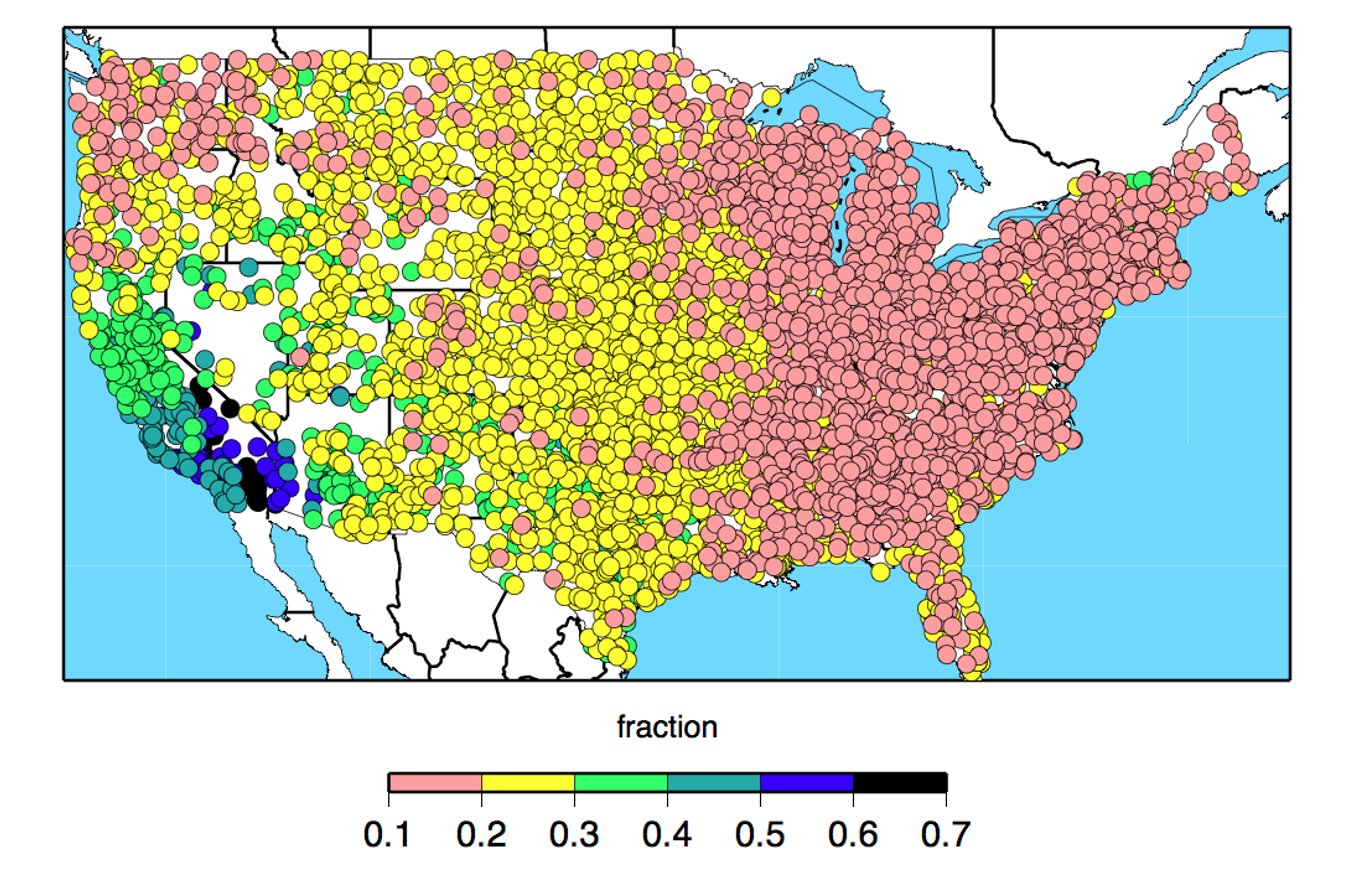
\includegraphics[width=0.8\textwidth,trim={0 0 0 0},clip=true]{Plots/ch1_coefficientofvariation.png}
	\caption{Coefficient of variation in total precipitation from 1951-2008. Reprinted from \protect\citeNP{dettinger2011atmospheric}}.
	\label{fig:coefvar}
\end{figure}

In addition to concerns with spatial extrapolation, there is temporal extrapolation. Climate change emposes \textbf{non-stationarity} in environmental variables like precipitation and temperature. Empirical models for flow should not be used to extrapolate beyond the limits of the variables the model observes or it will risk large errors. However, many advances in time-series analysis handle non-stationarity in data; one can reduce the process to a stationary one (i.e., trend seasonality and noise can be decomposed) or consider these processes as stochastic.
% Jay's comment: I have always thought that climate change makes empirical models riskier. But perhaps there are benefits of taking/modifying empirical models of warmer basins for todays cooler basins. 

Another downside is the \textbf{complexity in model structure}, especially in ensemble statistical learning methods, sometimes referred to as black-box models. If inference, or model parameters, are of interest, complex models introduce challenges. Dimensionality reduction methods (e.g., principle component analysis, partial least squares) and regularization techniques in regression (e.g., ridge, lasso, and elastic net) can help reduce the number of model parameters, and systematically produce simpler models \cite{friedman2001elements}. 

The essential \textbf{arbitrariness in the selection of the form} of an empirical model is another drawback \cite{klemes1982empirical}. Most studies report using one modeling method, which perhaps suggests that researchers are not employing more than one modeling method. Such a study could provide insights into the system by revealing the sensitivity of results to the algorithms employed. Therefore, the application and comparison of different machine learning models to the PUB problem was considered in this study. 

Lastly, some limitations are caused by the \textbf{nature of the algorithms} deployed. For example, regression-based random forest models make predictions by averaging predictions made by multiple regression trees. Therefore, the ensemble model limits the predictions it makes to the range seen in the training data; the predictions do not extrapolate to ranges not seen in the training data. In fact, averaging dampens the density function when we compare  observed to predicted data. This is especially problematic where the extreme tails of the distribution (i.e., floods and droughts) are of interest. Another example is that of the SVMs mentioned before that seem to perform poorly on low rainfall data. 

% some of these models get it right for the wrong reasons, and those few statistics are not reflective of how well a model does, two models can have the same statistics but perform vastly differently. 

%----------------------------------------------------------------------------------------------------------------------------------------------------------------------------------------------------------
\section{Conclusion} 
Generally, in statistical learning, applications lag behind advances in theory; the application of statistical learning theory to water resources problems is still in the bulldozer era, so, most models are computationally expensive. In the past two decades, in hydrology, statistical learning methods have been applied to modeling rainfall-runoff processes, predicting streamflow temperatures, sediment and nutrient loadings, forecasting the groundwater heads in an aquifer, or water demand among many others.

This chapter's main contribution is a heuristic guide to empirical model selection. Like a flowchart, it guides in selecting methods tailored to general purposes and limitations of various empirical modeling approaches. This guide should help in selecting from range of possible methods that are well suited to a problem at hand and give some comparative insights on these diverse methods. As a heuristic it works in most cases, but it is not comprehensive or applicable to all problems. 

In some cases, a wide range of empirical models can be employed, suggesting that no one single modeling method is useful across all locations, timescales, and problems. Also, despite their other limitations discussed in this chapter, these methods are much easier, faster, and less expensive to apply and study than mechanistic models. They are well suited to dynamic, non-linear and sometimes noisy data, especially when underlying physical processes are complex or not fully understood. In addition, the purpose of modeling is often to inform decision makers with adequate timing. For example, models need to be run during and just before flood events. Real-time applications require rapid computation, which statistical methods provide. The merits of statistical learning techniques, as a subset of empirical models, motivate their study in the following chapters.

This dissertation follows steps outlined in Figure \ref{fig:steps}. Chapter two compares two different data transformations that reflect our philosophical view of hydrology. Chapter three explores the effect of the loss functions on the model parameters and estimates. Chapter four compares different resampling methods for test error approximation. Chapter five discusses model development for non-stationary hydrologic processes. 

\begin{figure}[H]
	\centering
	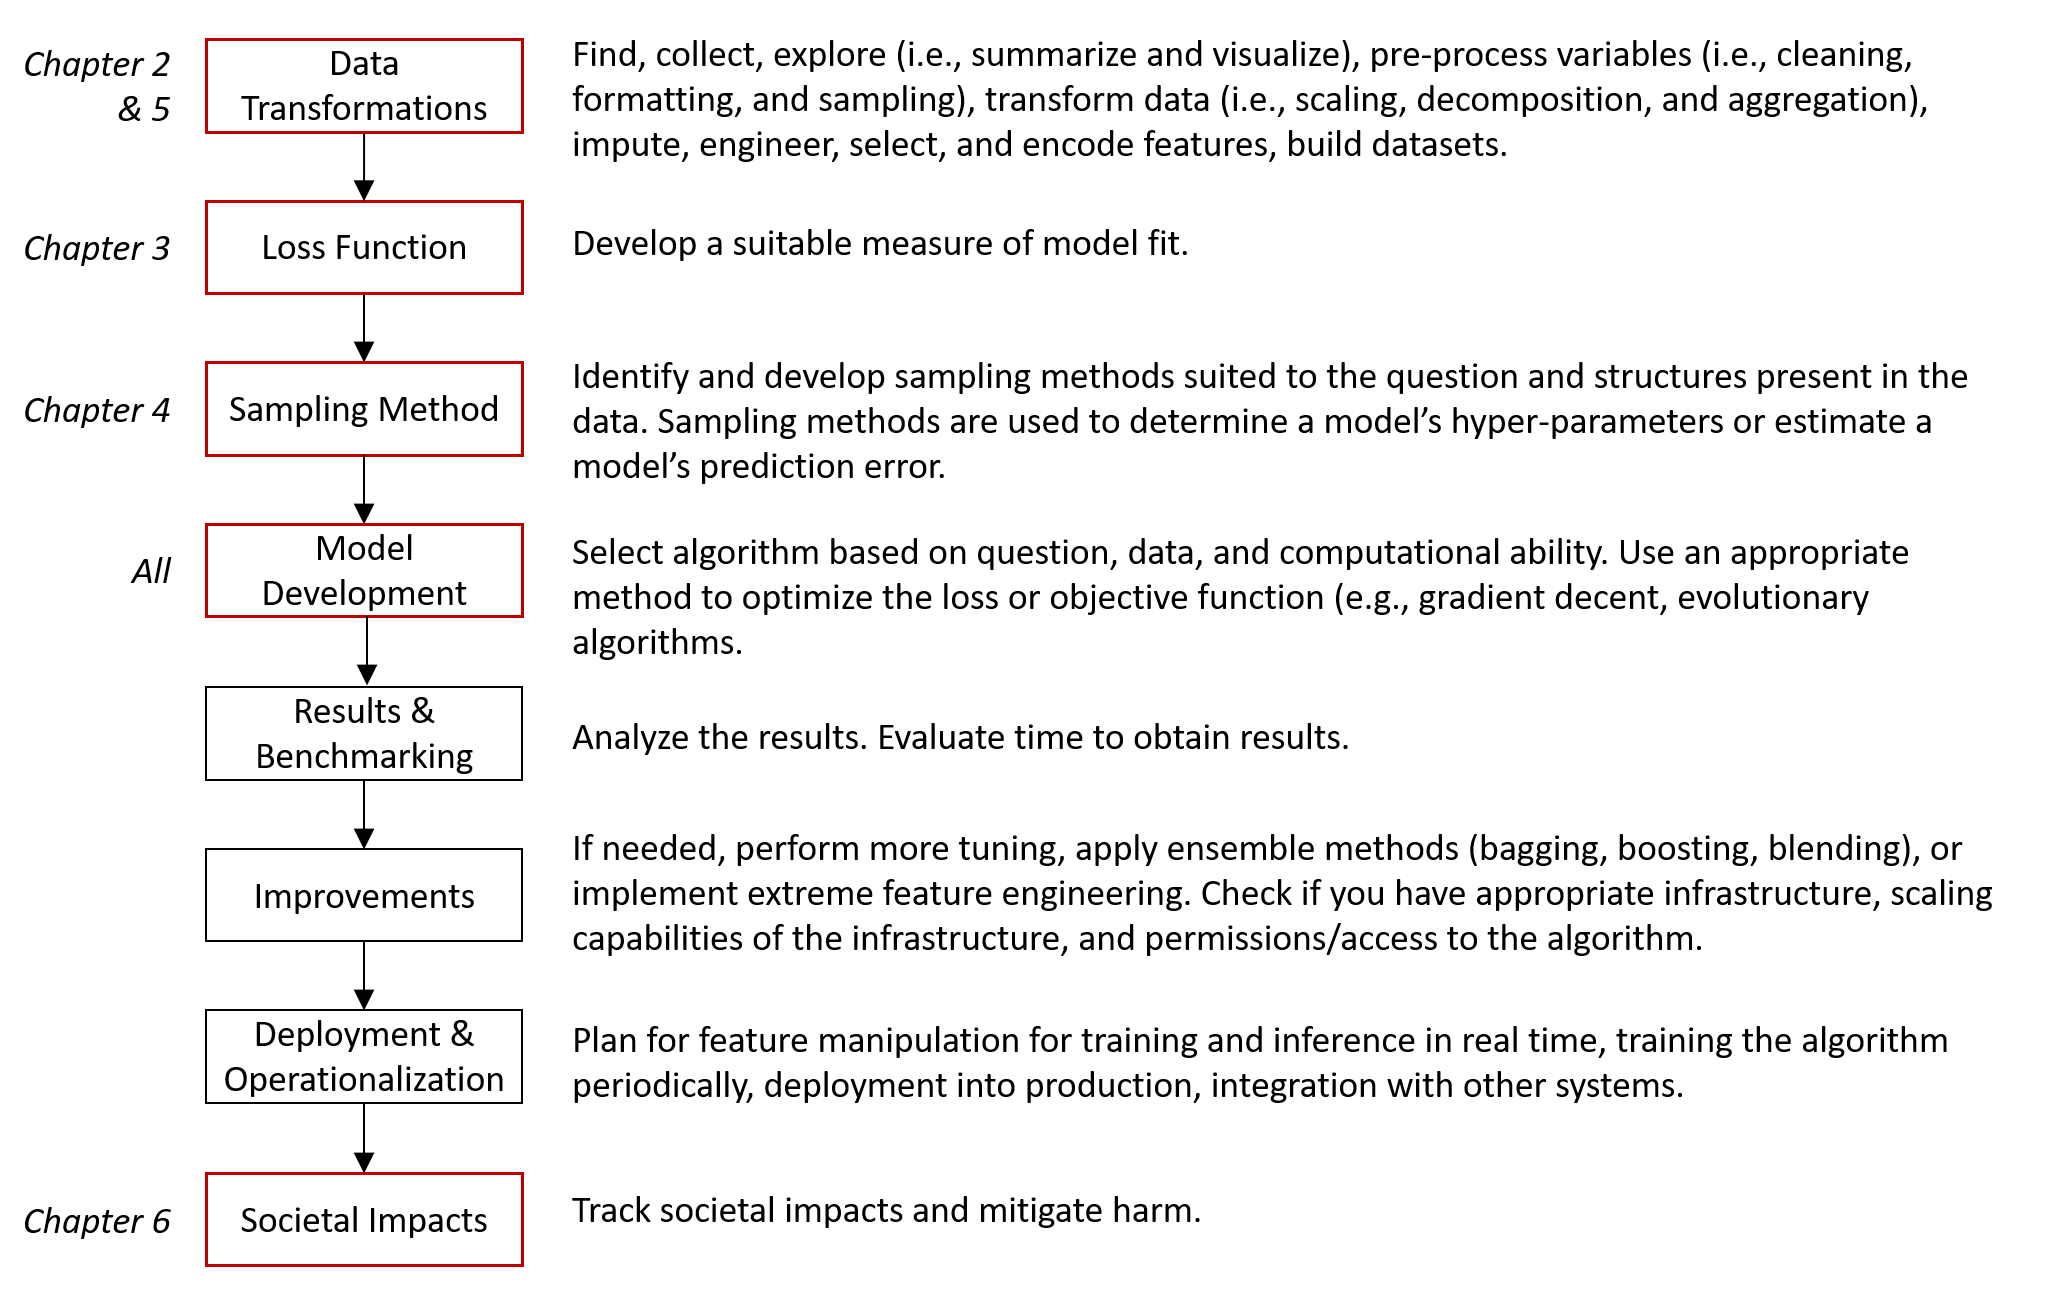
\includegraphics[width=\textwidth,trim={0 0 0 0},clip=true]{plots/ch1_diss_steps.png}
	\caption{Statistical learning steps. Adapted from \protect\citeNP{mlmastery2014, mindmap2017}. Each chapter of this dissertation discusses a unique step.} 
	\label{fig:steps}
\end{figure}

%\begin{enumerate}
%	\item Data: Find, collect, explore (i.e., summarize and visualize), pre-process variables (i.e., cleaning, formatting, and sampling), transform data (i.e., scaling, decomposition, and aggregation), impute, engineer, select, and encode features, build datasets.
%	\item Model: Select algorithm based on question and available data.
%	\item Loss or objective function: Develop a measure of model fit.
%	\item Optimization: Use an appropriate method to optimize the loss or objective function (e.g., gradient decent, evolutionary algorithms).
%	\item Tuning: Determine the model's hyper-parameters with cross-validation. There are multiple methods (e.g., grid search or random search) for optimal hyper-parameter specification. 
%	\item Results and Benchmarking: Analyze the results. Evaluate time to obtain results.
%	\item Improvements: If needed, perform more tuning, apply ensemble methods (bagging, boosting, blending), or implement extreme feature engineering.
%	\item Scaling: Check if the algorithm scales for expanding training datasets and in cases of inference.
%	\item Deployment and Operationalization: Plan for feature manipulation for training and inference in real time, training the algorithm periodically, deployment into production, integration with other systems.
%	\item Infrastructure: Check if you have appropriate infrastructure, scaling capabilities of the infrastructure, and permissions/access to the algorithm.
%\end{enumerate}

%Research objectives of this dissertation include:
%
%\begin{itemize}
%	\item \textit{Chapter 2, Data Transformations: Philosophical Views of Hydorlogic Modeling} - Present different data transformation techniques for hydrologic modeling that each represent a different philosophical view of hydrologic processes. 
%	\item \textit{Chapter 3, Rethinking Resampling Methods} - Describe how to more accurately estimate a model's prediction error with resampling methods when the data is structured. Structured data has internal correlation structures that need to be accounted for when resampling. 
%% \textbf{Questions}: How can we accurately estimate the model's prediction error with resampling methods when the data is structured? Structured data has internal correlation structures that need to be accounted for when resampling. \\
%	\item \textit{Chapter 4, New Loss Functions} - Encourage examination of off-the-shelf machine learning methods, specifically their default objective function. Identify some characteristics to consider when designing a loss function for machine learning algorithms. Examine how different loss functions perform when used to model hydrology. 
%% \textbf{Questions}: What are some characteristics one should consider when designing a loss function for machine learning algorithms? How do different loss functions perform when they are used to model hydrology? \\
%%What are some possible alternatives to the objective functions typically applied in off-the-shelf statistical learning techniques? These alternatives should be more suited to modeling extremes, which is usually where good management is more paramount in water resources. \\
%	\item \textit{Chapter 5, Modeling Methods} - Discuss the methods used for hydrologic modeling and their performance.  
%	\item \textit{Chapter 6, Climate Change Considerations} - Discuss data processing and modeling changes to incorporate a changing hydrology.
%	\item \textit{Chapter 7, Beyond McDonaldization: The ``Robotanization" of Agriculture} - Look to the impacts of statistical learning on our society and economy. Discuss how statistical learning is changing our society and what ``irrationalities" may it produce or take away that make it distinct from past mechanization. 
%% \textbf{Questions}: How is statistical learning changing our society? In other words, what ``irrationalities" may it produce that may have been non-existent in past mechanization, and what irrationalities may it take away? \\
%\end{itemize}




	
